\documentclass{article}
\usepackage{tikz}
\usepackage{amsmath}

\begin{document}

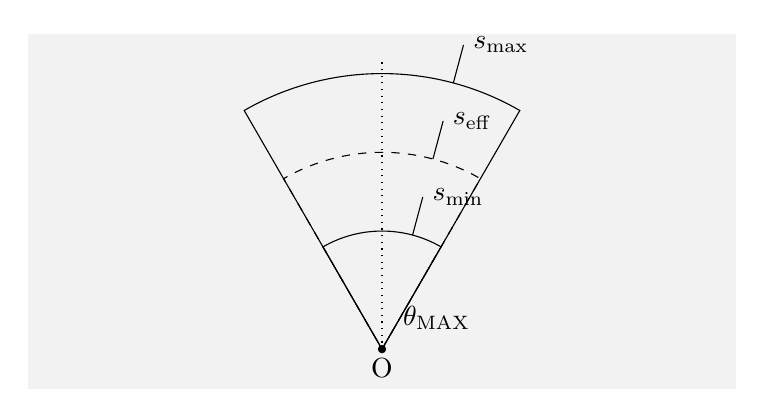
\begin{tikzpicture}
% Define parameters
\def\smin{1.5}    % Minimum comoving distance
\def\seff{2.5}    % Effective comoving distance
\def\smax{3.5}    % Maximum comoving distance
\def\thetamax{60} % Half-opening angle in degrees

% Background rectangle
\fill[gray!10] (-4.5,-0.5) rectangle (4.5,4);

% Origin
\coordinate (O) at (0,0);
\node[below] at (O) {O};
\fill (O) circle (1.5pt);

% Draw the spherical cap boundaries
\draw (O) -- (\thetamax:\smin) arc (\thetamax:180-\thetamax:\smin) -- (O);
\draw (O) -- (\thetamax:\smax) arc (\thetamax:180-\thetamax:\smax) -- (O);

% Draw the effective distance (dashed)
\draw[dashed] (O) -- (\thetamax:\seff) arc (\thetamax:180-\thetamax:\seff) -- (O);

% Draw central axis (dotted)
\draw[dotted] (0,0) -- (0,\smax+0.2);

% Draw angle marker (dotted)
\draw[dotted] (0,0) -- (\thetamax:2);

% Label the angle
\node at (\thetamax/2:0.8) {$\theta_\mathrm{MAX}$};

% Label the distances
\draw (\thetamax+15:\smin) -- (\thetamax+15:\smin+0.5) node[right] {$s_\mathrm{min}$};
\draw (\thetamax+15:\seff) -- (\thetamax+15:\seff+0.5) node[right] {$s_\mathrm{eff}$};
\draw (\thetamax+15:\smax) -- (\thetamax+15:\smax+0.5) node[right] {$s_\mathrm{max}$};

\end{tikzpicture}

\end{document}